% mainfile: ../../main.src.tex
\chapter{Theory of spectral noise estimation}\label{ch:speck:theory}
\mylettrine{T}{here} exists a multitude of methods for estimating noise properties of a classical signal $x(t)$.\sidenote{
    We discuss only classical noise here, meaning $x(t)$ commutes with itself at all times. For descriptions of and spectroscopy protocols for quantum noise refer to \citerr{Clerk2010}{Paz-Silva2017}, for example.
}
\todo{lay out some others}

If the noisy process $x(t)$ has Gaussian statistics, meaning that the value at a given point in time follows a normal distribution with some mean $\mu$ and variance $\sigma^2$ over multiple realizations of the process, it can be fully described by the \gls{psd} $S(\omega)$.\sidenote{
    \label{sidenote:speck:theory_vocabulary}
    The term \emph{power spectrum} is often used interchangably.
    I will do so as well, but emphasize at this point that in digital signal processing in particular, the \emph{spectrum} is a different quantity from the \emph{spectral density}.
    See also \cref{sidenote:speck:software_vocabulary} in \cref{ch:speck:software}.
}
\todo{maybe a classical signal processing ref?}
For the purpose of noise estimation, the assumption of Gaussianity is a rather weak one as the noise typically arises from a large ensemble of individual fluctuators and is therefore well approximated by a Gaussian distribution by the central limit theorem.\sidenote{
    As an example, consider electronic devices, where voltage noise arises from a large number of defects and other charge traps in oxides being populated and depopulated at certain rates $\gamma$. The ensemble average over these so-called \glspl{tlf} then yields the well-known \oneoverf-like noise spectra (at least for a large density~\cite{Mehmandoost2024}).
}
\todo{flesh out this sidenote?}
Even if the process $x(t)$ is not perfectly Gaussian, non-Gaussian contributions can be seen as higher-order contributions if viewed from the perspective of perturbation theory, and therefore the \gls{psd} still captures a significant part of the statistical properties.
For this reason, the \gls{psd} is the central quantity of interest in noise spectroscopy and I will discuss some of its properties in the following.

For real signals $x(t) \in\mathbb{R}$, $S(\omega)$ is an even function and one therefore distinguishes the \emph{two-sided} \gls{psd} $S^{(2)}(\omega)$ defined over $\mathbb{R}$ from the \emph{one-sided} \gls{psd} $S^{(1)}(\omega) = 2 S^{(2)}(\omega)$ defined only over $\mathbb{R}^+$.
Complex signals $x(t)\in\mathbb{C}$ such as those generated by Lock-in amplifiers after demodulation in turn have asymmetric, two-sided \glspl{psd}.
\todo{flesh out}

\section{Spectrum estimation from time series}\label{sec:speck:theory:time_series_estimation}
To see how the \gls{psd} may be estimated from time-series data, consider a continuous wide-sense stationary\sidenote{
    For a wide-sense stationary (also called weakly stationary) process $x(t)$, the mean is constant and the auto-correlation function $C(t, t') = \ev{x(t)\conjugate x(t^\prime)}$ is given by $\ev{x(t)\conjugate x(t + \tau)} = \ev{x(0)\conjugate x(\tau)}$ with $\tau = t^\prime - t$.
    That is, it is a function of only the time lag $\tau$ and not the absolute point in time.
    For Gaussian processes as discussed here, this also implies stationarity~\cite{Koopmans1995}.
    The property further implies that $C(\tau)$ is an even function.
}
\todo{sketch of auto-correlation function?}
signal in the time domain $x(t)\in\mathbb{C}$ that is observed for some time $T$.
We define the windowed Fourier transform of $x(t)$ and its inverse by\sidenote{
    In this chapter we will always denote the Fourier transform of some quantity $\xi$ using the same symbol with a hat, $\hat{\xi}$.
}
\begin{align}
    \hat{x}_T(\omega) &= \int_{0}^{T}\dd{t} x(t)\e^{-\i\omega t} \label{eq:speck:windowed_ft}\\
       \qq*{and} x(t) &= \intinf\ddf{\omega}\hat{x}_T(\omega)\e^{\i\omega t}, \label{eq:speck:windowed_ft:inverse}
\end{align}
\ie, we assume that outside of the window of observation $x(t)$ is zero.
The auto-correlation function of $x(t)$ is given by
\begin{align}
    C(\tau) &= \expval{x(t)\conjugate x(t + \tau)} \label{eq:speck:autocorrelation}\\
            &= \lim_{T\to\infty} \frac{1}{T}\int_0^T\dd{t} x(t)\conjugate x(t + \tau),
\end{align}
where $\expval{\placeholder}$ is the ensemble average over multiple realizations of the process and the last equality holds true for ergodic processes.
Expressing $x(t)$ in terms of its Fourier representation (\cref{eq:speck:windowed_ft}) and reordering the integrals, we get\sidenote{
    Mathematicians might at this point argue the integrability of $x(t)$, but as we deal with physical processes with finite bandwidth (and have no shame), we do not.
}
\begin{align}
    C(\tau) &= \lim_{T\to\infty}\frac{1}{T}\int_0^T\dd{t}
                \intinf\ddf{\omega}\hat{x}_T(\omega)\conjugate\e^{-\i\omega t}
                \intinf\ddf{\omega^\prime}\hat{x}_T(\omega^\prime)\e^{\i\omega^\prime (t + \tau)}  \\
            &= \lim_{T\to\infty}\frac{1}{T}\intinf\ddf{\omega}\intinf\ddf{\omega^\prime}
                \hat{x}_T(\omega)\conjugate\hat{x}_T(\omega^\prime)\e^{\i\omega^\prime\tau}
                \int_0^T\dd{t}\e^{\i t (\omega^\prime - \omega)} \label{eq:speck:autocorrelation:fourier}
\end{align}
The innermost integral approaches a $\delta$-function for large $T$,\sidenote{
    Note that, because $x(t)$ is wide-sense stationary, we may shift the limits of integration $\int_{0}^{T}\to\int_{-\flatfrac{T}{2}}^{+\flatfrac{T}{2}}$.
}
allowing us to further simplify this under the limit as
\begin{align}
    C(\tau) &= \lim_{T\to\infty} \frac{1}{T}\intinf\ddf{\omega}\intinf\ddf{\omega^\prime}
                \hat{x}_T(\omega)\conjugate\hat{x}_T(\omega^\prime)
                \e^{\i\omega^\prime\tau}\delta(\omega^\prime - \omega)\\
            &= \lim_{T\to\infty}\frac{1}{T}
                \intinf\ddf{\omega}\abs{\hat{x}_T(\omega)}^2 \e^{\i\omega\tau} \\
            &= \intinf\ddf{\omega} S(\omega) \e^{\i\omega\tau} \label{eq:speck:wiener_khinchin}
\end{align}
with the \gls{psd}
\begin{align}
    S(\omega) &= \lim_{T\to\infty}\frac{1}{T}\abs{\hat{x}_T(\omega)}^2 \label{eq:speck:psd:definition}\\
              &= \intinf\dd{\tau} C(\tau)\e^{-\i\omega\tau}
\end{align}
\Cref{eq:speck:wiener_khinchin} is the Wiener-Khinchin theorem that states that the auto-correlation function $C(\tau)$ and the \gls{psd} $S(\omega)$ are Fourier-transform pairs~\cite{Koopmans1995}.
Furthermore, defining the latter through \cref{eq:speck:psd:definition} gives us an intuitive picture of the \gls{psd} if we recall Parseval's theorem,
\begin{align}\label{eq:speck:parseval}
    \intinf\ddf{\omega}\frac{1}{T}\abs{\hat{x}_T(\omega)}^2 = \frac{1}{T}\intinf\dd{t}\abs{x(t)}^2.
\end{align}
That is, the total power $P$ contained in the signal $x(t)$ is given by integrating over the \gls{psd}.
Similarly, the power contained in a band of frequencies $[\omega_1, \omega_2]$ is given by
\begin{align}
    P(\omega_1, \omega_2) &= \rms_S\left(\omega_1, \omega_2\right)^2 \label{eq:speck:psd:bandpower}\\
                          &= \int_{\omega_1}^{\omega_2}\ddf{\omega} S(\omega)
\end{align}
where $\rms_S\left(\omega_1, \omega_2\right)$ is the \acrlong{rms} within this frequency band.
These relations are helpful when analyzing noise \glspl{psd} to gauge the relative weight of contributions from different frequency bands to the total noise power.

\Cref{eq:speck:psd:definition} represents the starting point for the experimental spectrum estimation procedure.
Instead of a continuous signal $x(t), t\in [0, T]$, consider its discretized version\sidenote{
    We only discuss the problem of equally spaced samples here. Variants for spectral estimation of time series with unequal spacing exist~\cite{Lomb1976,Scargle1982}.
}
\begin{align}\label{eq:speck:signal:discrete}
    x_n \qc n\in\lbrace 0, 1, \dotsc, N - 1\rbrace
\end{align}
defined at times $t_n = n\Delta t$ with $T = N\Delta t$ and where $\Delta t = \fs\inverse$ is the sampling interval (the inverse of the sampling frequency \fs).
Invoking the ergodic theorem, we can replace the long-term average in \cref{eq:speck:psd:definition} by the ensemble average over $M$ realizations $i$ of the noisy signal $x_n\gth{m}$ and write
\begin{align}\label{eq:speck:psd:bartlett}
    S_n &= \frac{1}{M} \sum_{i=0}^{M-1} \abs{\hat{x}_n\gth{m}}^2 \\
        &= \frac{1}{M} \sum_{i=0}^{M-1} S_n\gth{m}
\end{align}
where $\hat{x}_n\gth{m}$ is the discrete Fourier transform of $x_n\gth{m}$, we defined the \emph{periodogram} of $x_n\gth{m}$ by
\begin{align}\label{eq:speck:periodogram}
    S_n\gth{m} = \abs{\hat{x}_n\gth{m}}^2,
\end{align}
and $S_n$ is an \emph{estimate} of the true \gls{psd} sampled at the discrete frequencies $\omega_n = \flatfrac{2\pi n}{T} \in 2\pi\times\lbrace\flatfrac{-\fs}{2}, \dotsc, \flatfrac{\fs}{2}\rbrace$.\sidenote{
    We blithely disregard integer algebra issues occuring here for conciseness and leave it as an exercise for the reader to figure out what the exact bounds of the set of $\omega_n$ are.
}
\Cref{eq:speck:psd:bartlett} is known as Bartlett's method~\cite{Bartlett1948} for spectrum estimation.\sidenote{
    \label{sidenote:continuum_limit}
    By taking the limit $M\to\infty$ one recovers the true \gls{psd}, \[\lim_{M\to\infty}S_n = S(\omega_n).\]
    The continuum limit is as always obtained by sending $\Delta t\to 0, N\to\infty, N\Delta t=\text{const}$.
}

To better understand the properties of this estimate, let us take a look at the parameters $\Delta t$, $N$, and $M$.
The sampling interval $\Delta t$ defines the largest resolvable frequency by the Nyquist sampling theorem,
\begin{align}\label{eq:speck:f_max}
    \fmax = \frac{\fs}{2} = \frac{1}{2\Delta t}.
\end{align}
In turn, the number of samples $N$ determines the frequency resolution $\Delta f$, or smallest resolvable frequency,
\begin{align}\label{eq:speck:f_min}
    \fmin = \Delta f = \frac{1}{T} = \frac{1}{N\Delta t} = \frac{\fs}{N}.
\end{align}
Lastly, $M$ determines the variance of the set of periodograms $\bigl\lbrace S_n\gth{m}\bigr\rbrace_{i=0}^{M-1}$ and hence the accuracy of the estimate $S_n$.

In practice, the ensemble realizations $i$ are of course obtained sequentially, implying that one acquires a time series of data $x_n, n\in\lbrace0, 1, \dotsc, NM - 1\rbrace$ and partitions these data into $M$ sequences of length $N$.
It becomes clear, then, that the Bartlett average (\cref{eq:speck:psd:bartlett}) trades spectral resolution (larger $N$) for estimation accuracy (larger $M$) given the finite acquisition time $T = NM\Delta t$.

An improvement in data efficiency can be obtained using Welch's method~\cite{Welch1967}.
To see how, we first need to discuss spectral windowing.

\section{Window functions}\label{sec:speck:theory:windows}
Partitioning a signal $x_n$ into $M$ sections $x_n\gth{m}$ of length $N$ is mathematically equivalent to multiplying the signal with the rectangular \emph{window function} given by\sidenote{
    This window is also known as the boxcar or Dirichlet window.
}
\begin{align}\label{eq:speck:window:boxcar}
    w_n\gth{m} =
    \begin{cases}
        1\qif (m - 1) N \leq n < m N\qand \\
        0\qelse
    \end{cases}
\end{align}
so that $x_n\gth{m} = x_n w_n\gth{m}$.
\todo{add $\omega_n\gth{m}$, scaled ticks}
\begin{marginfigure}
    \centering
    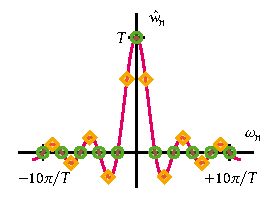
\includegraphics{pdf/spectrometer/rect}
    \caption{The Fourier representation of the rectangular window in continuous time.}
    \label{fig:boxcar_fourier}
\end{marginfigure}
Now recall that multiplication and convolution are duals under the Fourier transform, implying that
\begin{align}\label{eq:speck:window:ft_pairs}
    \hat{x}_n\gth{m} = \hat{x}_n \ast \hat{w}_n\gth{m}.
\end{align}
where the Fourier representation of the rectangular window\sidenote{
    $\sinc(x) = \flatfrac{\sin(x)}{x}$.
}
\begin{align}
    \hat{w}_n\gth{m} &= \hat{w}_n \e^{-\i(m - \flatfrac{1}{2})\omega_n T}, \label{eq:speck:window:boxcar:fourier}\\
             \hat{w}_n &= T\sinc\left(\frac{\omega_n T}{2}\right). \label{eq:speck:window:boxcar:fourier:unshifted}
\end{align}
\Cref{fig:boxcar_fourier} shows the unshifted rectangular window $\hat{w}_n$ in Fourier space.
We can hence understand the Fourier spectrum of $x_n\gth{m}$ as sampling $\hat{x}_n$ with the probe $\hat{w}_n\gth{m}$.
However, while in the continuum limit (\cf \cref{sidenote:continuum_limit}) \cref{eq:speck:window:boxcar:fourier:unshifted} tends towards $\delta(\omega_n)$ and thus will produce a faithful reconstruction of the true spectrum, the finite frequency spacing $\Delta f$ of discrete signals introduces a finite bandwidth of the probe as well as \emph{sidelobes}.
These effects induce what is known as \emph{spectral leakage}~\cite{Harris1978,Koopmans1995} and lead to artifacts and deviations of the spectrum estimator $S_n$ from the true spectrum $S(\omega_n)$.

For this reason, a plethora of \emph{window functions} have been introduced to mitigate the effects of spectral leakage.
Key properties of a window are the spectral bandwidth (center lobe width) and sidelobe amplitude between which there typically is a tradeoff.\sidenote{
    Wikipedia gives a good overview of existing window functions~\cite{WindowFunctionWiki}.
}
\todo{add $\omega_n\gth{m}$, scaled ticks}
\begin{marginfigure}
    \centering
    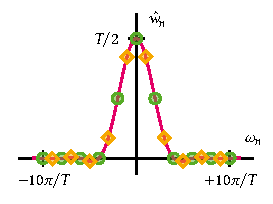
\includegraphics{pdf/spectrometer/hann}
    \caption{The Fourier representation of the Hann window in continuous time.}
    \label{fig:hann_fourier}
\end{marginfigure}
A window frequently used in spectral analysis is the Hann window~\cite{Nuttall1981},
\begin{align}\label{eq:speck:window:hann}
    w_n\gth{m} =
    \begin{cases}
        \cos^2\left(\frac{\pi n}{N}\right)\qif (m - 1)N\leq n < mN\qand \\
        0\qelse
    \end{cases}
\end{align}
with the Fourier representation of the unshifted window,
\begin{align}\label{eq:speck:window:hann:fourier_unshifted}
%    \hat{w}_n &= \frac{2T\pi^2\sinc(\flatfrac{\omega_n T}{2})}{4\pi^2 - \omega_n^2 T^2},
%    \hat{w}_n &= \frac{2\pi^2 T\sinc(\flatfrac{\omega_n T}{2})}{(2\pi - \omega_n T)(2\pi + \omega_n T)},
    \hat{w}_n &=  T\sinc\left(\frac{\omega_n T}{2}\right)\times
                    \frac{1}{2(1 - \flatfrac{\omega_n T}{2\pi})(1 + \flatfrac{\omega_n T}{2\pi})},
\end{align}
shown in \cref{fig:hann_fourier}.
The favorable properties of the Hann window are apparent when compared to the rectangular window in \cref{fig:boxcar_fourier}; the sidelobes are quadratically suppressed while the center lobe is only slightly broadened.

Another favorable property of the Hann window is that $w_0\gth{0} = w_{N-1}\gth{0} = 0$.
This suppresses detrimental effects arising from a possible discontinuity ($x_0\gth{0}\neq x_{N-1}\gth{0}$) at the edge of a data segment related to the discrete Fourier transform, which assumes periodic data.\sidenote{
    Although this can usually also be achieved by detrending the data before performing the Fourier transform, which is a good idea in any case.
}

\section{Welch's method}\label{sec:speck:theory:welch}
Contemplating \cref{eq:speck:window:hann}, one might come to the conclusion that using a window such as this is not very data efficient in the sense that a large fraction of samples located at the edge of the window is strongly suppressed and hence does not contribute significantly to the spectrum estimate.
To alleviate this lack of efficiency, one can introduce an overlap between adjacent data windows.
That is, instead of partitioning the data $x_n$ into $M$ non-overlapping sections of length $N$, one shifts the $m$th window forward by $-mK$ with $K>0$ the overlap.
Finally, the periodogram (\cref{eq:speck:periodogram}) is computed for each window and subsequently averaged to obtain the spectrum estimator (\cref{eq:speck:psd:bartlett}).

This method of spectrum estimation is known as Welch's method~\cite{Welch1967}.
One can show~\cite{Welch1967} that the correlation between the periodograms of adjacent, overlapping windows is sufficiently small to avoid a biased estimate.
The overlap naturally depends on the choice of window; a typical value for the Hann window $K = \flatfrac{N}{2}$ with which one would obtain $M = \flatfrac{2L}{N} - 1$ windows for data of length $L$.\sidenote{
    Again neglecting integer arithmetic issues.
}
\begin{figure}[tphb]
    \centering
    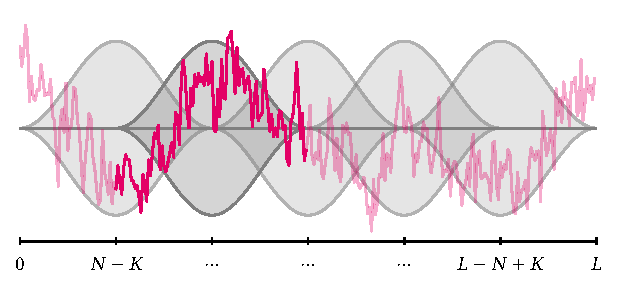
\includegraphics[width=\textwidth]{pdf/spectrometer/welch}
    \caption{
        Illustration of Welch's method for spectrum estimation.
        The data (pink) of length $L$ is partitioned into $K = \flatfrac{2L}{N} - 1$ segments of length $N$.
        Each segment is multiplied with a window function (gray) which reduces spectral leakage and other artifacts.
        A finite overlap $K$ between adjacent windows (gray) ensures efficient sample use.
    }
    \label{fig:welch}
\end{figure}

\Cref{fig:welch} conceptually illustrates Welch's method for a trace of \oneoverf noise with $L = 300$ samples in total.
Choosing the Hann window and an overlap of \qty{50}{\percent} results in $M=5$ segments for a window length of $N=100$.
The data in the second window is highlighted.

\subsection{Parameters}\label{subsec:speck:theory:welch:parameters}
\begin{margintable}
    \centering
    \footnotesize
    \caption[Overview of spectrum estimation parameters]{
        Overview of spectrum estimation parameters.
        The parameters can be assigned into three groups
        \begin{enumerate*}[
            before=\unskip{: }, itemjoin={{, }}, itemjoin*={{, and }}
        ]
            \item \acrshort{daq} parameters configuring the data acquisition device
            \item Welch parameters specifying the periodogram averaging
            \item Spectrum properties induced by the above
        \end{enumerate*}.
    }
    \label{tab:parameters}
    \begin{tabularx}{\marginparwidth}{ c l }
        \multicolumn{2}{l}{1. \acrshort{daq} parameters} \\
        \toprule
        $L$ & Total number of samples \\
        \fs & Sample rate \\
        [0.5ex]
        \multicolumn{2}{l}{2. Welch parameters} \\
        \toprule
        $K$ & Number of overlap samples \\
        $N$ & Number of segment samples \\
        $M$ & Number of Welch segments \\
        [0.5ex]
        \multicolumn{2}{l}{3. Spectrum parameters} \\
        \toprule
        \fmin & Smallest resolvable frequency \\
        \fmax & Largest resolvable frequency \\
    \end{tabularx}
\end{margintable}

We are now in a position to discuss how the various parameters of a time series relate to both to physical parameters of the resulting spectrum estimate and to each other.
To this end, we will go through the typical procedure of acquiring a spectrum estimate using Welch's method chronologically.

To acquire data using some form of (digital) \gls{daq}, one usually needs to specify two parameters first: the total number of samples to be acquired, $L$, and the sample rate, \fs.
This results in a measurement of duration $T = L\Delta t$ where $\Delta t = \fs\inverse$ as previously mentioned.
The choice of \fs already induces an upper bound on the first parameter characterizing the \gls{psd} estimate: the largest resolvable frequency $\fmax\leq\flatfrac{\fs}{2}$ (\cf \cref{eq:speck:f_max}, but note that we allow \fmax to be smaller than half the sample rate in anticipation of hardware constraints).
Next, we choose a number of Welch averages, $M$, \ie, data partitions, and their overlap, $K$.
In doing so, one fixes the number of samples per partition $N$ and thereby induces the lower bound on the second parameter characterizing the \gls{psd} estimate: the frequency spacing $\df = \flatfrac{1}{N} \leq \fmin$ (\cf \cref{eq:speck:f_min}).\sidenote{
    Technically, the smallest resolvable frequency in a \gls{fft} is zero, of course. But as data is typically detrended (a constant or linear trend subtracted) before computation of the periodogram, the smallest \emph{meaningful} frequency is given by \fmin.
}
\todo{D(A)G for parameter interdependencies?}
